\chapter{An Event Streams Composition Model}
\label{ch3}
\textit{This chapter presents the building blocks to model an event composition system. It defines events, which are the entities manipulated by such a system. Then, it introduces event 
streams and stream based operations. Then it defines how to represent an event composition, with the related QoS dimensions.}
\vspace{5cm}
\vspace{2ex}\vfill
\minitoc

%\section{Introduction}
 %\label{ch3:intro}
% A vast number of event management models and systems have been, and continues to be proposed. Several standardization efforts are being made to specify how entities can export the structure and data transported by events. Models proposed in the literature range from simple models which describe the notification of signals, to evolved models which take into account various policies to manage and compose events. 
% Existing models have been defined in an ad hoc way, notably linked to the application context (active DBMS event models), or in a very general way in middleware (Java event service, MOMs). Of course, customizing solutions prevents systems to be affected with the overhead of an event model way too sophisticated for their needs. However, they are not adapted when the systems evolve, cooperate and scale, leading to a lack of adaptability and flexibility. 
% This chapter introduces the concepts of event, event type and event streams. It introduces stream based operations and presents how to define an event composition expression. It ends with the specification of QoS related to an event composition expression.  
%It introduces the notion of priority that can be associated to events in some particular contexts.

\section{Event, event type, event streams}
\label{ch3:sec2}
A vast number of event management models and systems have been, and continues to be proposed. Several standardization efforts are being made to specify how entities can export the structure and data transported by events. Models proposed in the literature range from simple models which describe the notification of signals, to evolved models which take into account various policies to manage and compose events. 
Existing models have been defined in an ad hoc way, notably linked to the application context (active DBMS event models), or in a very general way in middleware (Java event service, MOMs). Of course, customizing solutions prevents systems to be affected with the overhead of an event model way too sophisticated for their needs. However, they are not adapted when the systems evolve, cooperate and scale, leading to a lack of adaptability and flexibility. 
%This chapter introduces the concepts of event, event type and event streams. It introduces stream based operations and presents how to define an event composition expression. It ends with the specification of QoS related to an event composition expression.
 \subsection{Definitions}
 \subsubsection{Preamble}
Let's assume a finite set of \textit{domains}, each consisting of a possibly infinite set of values. In particular, we consider the domain $\mathbb{S}$ of strings, $\mathbb{B}$ of booleans ($\{true, false\}$), $\mathbb{Z}$ of integers, and $\mathbb{R}$ of real numbers. We also consider a domain $\mathbb{T}$ defined by the set $\mathbb{N} \bigcup \{0\}$, i.e. the set of natural numbers plus zero, which characterizes time values. These can be represented alternatively as \textit{string, boolean, integer, real} and \textit{time} respectively. In addition, we assume a set   $\mathbb{A} = \{A_1,\ A_2,\ ...\}\ \subseteq\ \mathbb{S}$ of type names. 
\subsubsection{Complex value types}
Complex value types are represented by lower-case letters with hats (e.g. \^{t}) and are defined by a pair $A : def$, where $A$ is the name of the type and $def$ its definition. In order to enable access to both components we assume the functions \textit{name} and \textit{def}, which given a type will return the respective component of the type. For instance, for the type \textit{Power : real, name(Power : real) = Power} whereas \textit{def(Power : real) = real}.
The set of all complex value types $\mathcal{T}$ is defined inductively as follows.
\begin{enumerate}
 \item if $D$ is a domain, then $A\ :\ D$ is an atomic type named $A$, where $A \in \mathbb{A}$;
 \item if \^{t} is a type, then $A\ :\ \{\hat{t}\}$ is a set type named $A$;
 \item if $\hat{t_1}, ..., \hat{t_n}$ are types with distinct names, then $A\ :\ \langle\hat{t_1}, ..., \hat{t_n}\rangle$ is a tuple type named A, and each $\hat{t_i}$ is an attribute type;
 \item if $\hat{t_1}$ and  $\hat{t_2}$ are types with distinct names, then $A\ :\ \hat{t_1} \oplus \hat{t_2}$ is the alternative type.  
\end{enumerate}
Every type $\hat{t} \ \in \ \mathcal{T} $  denotes a set of complex value instances $\llbracket \hat{t} \rrbracket$ which is defined inductively as follows.
\begin{enumerate}
 \item For each atomic type $A\ :\ D$, $\llbracket A\ :\ D\rrbracket = \{d\ |\ d \in D\}$, where we assume the values of the domain $D$ given;
 \item for set types of the form $A\ :\ \{\hat{t}\}$, $\llbracket A\ :\ \{\hat{t}\}\rrbracket$ = $\{S\ |\ S\in\  \mathcal{P}(\llbracket \hat{t}\rrbracket)\}$, where $\mathcal{P}$ denotes the power set;
 \item for tuple types of the form $A\ :\ \langle  \hat{t_1}, ..., \hat{t_n}\rangle$, $\llbracket A\ : \ \langle  \hat{t_1}, ..., \hat{t_n}\rangle \rrbracket$ = $\{\langle v_1, ..., v_n\rangle \ | \ :\ v_i \in \llbracket \hat{t_i}\rrbracket \ \bigwedge \ i \ \in \ [1..n]\}$;
 \item for alternative type of the form $A\ :\ \hat{t_1} \oplus \hat{t_2}$, $\llbracket A\ :\   \hat{t_1} \oplus \hat{t_2} \rrbracket$ = $\{v\ |\ v \in \llbracket \hat{t_1}\rrbracket\ \bigvee\ v \in \llbracket \hat{t_2}\rrbracket\}$
\end{enumerate}
\subsubsection{Access to components of complex value instances}
We note $t\ \equiv\ \hat{t}$, to define an instance of a complex value type $\hat{t}$ named $t$. 
We define the function \textit{val} to obtain the value $v$ associated to an instance $t$. In addition, for tuple values $t$ of the type $A\ :\ \langle  \hat{t_1}, ..., \hat{t_n}\rangle$ such that $name(\hat{t_i})\ =\ A_i$, we adopt the dot notation $t.A_i$ to access the instance of the attribute type $\hat{t_i}$ of $t$. In particular, if we have $t = \langle v_1, ..., v_n\rangle$, then $\forall i \ \in \ [1..n],\ v_i\ =\ val(t.A_i)$.  
For example, $t\ \equiv Account\ :\ \langle id: string,\ balance: real\rangle$ denotes an instance $t$ of the tuple type $Account\ :\ \langle id: string,\ balance: real\rangle$. In addition, if $t = \langle B14,\ 500\rangle$ then, $val(t.id) = B14$ and $val(t.balance) = 500$.

For simplicity, we also adopt the notation $t$, to refer to the value $val(t)$ of an instance $t$. The difference between the value of the instance and the instance itself depends on the context.
For example, for the tuple instance $t= \langle B14,\ 500\rangle$ of the type $Account\ :\ \langle id: string,\ balance: real\rangle$, we have $t.id = B14$ and $t.balance = 500$.
 \subsection{Event}
 An event is something that happens at a particular place and time and that is particularly significant, interesting or unusual. In computing systems the notion of event has a major importance since it provides a powerful abstraction to model dynamic aspects of applications. For instance, events can represent state changes in databases; signals in message systems; changes of existing objects or the creation of new objects in object-oriented systems; or “real-world” events such as the departure or arrival of vehicles. In event-driven programming an event is a message that indicates a situation that happened, such as a keystroke or a mouse click. In process control an event is an occurrence that happened and that has been registered.  Examples are a purchase order, an email confirmation of an airline reservation, a stock tick message that reports a stock trade.
 
 The literature proposes different definitions of an event. For example, in \cite{Mansouri97gem} an event is a happening of interest, which occurs instantaneously at a specific time. Another definition given by \cite{Rosenblum97} characterizes an event as the instantaneous effect of the termination of an invocation of an operation on an object. According to the first definition, an event exists because some entity is interested in it; the second one defines events independently of any interested party. The second definition also subsumes an object model while the first one is neutral with respect to the model adopted for entities. 
% 
% In this document we define an event in terms of a source named producer in which the event occurs, and a consumer for which the event is significant (figure 2.1). Thus, an event describes a fact, a situation, observable in a producer and significant for a consumer.
% \begin{figure}[H]
%   \begin{center}
%     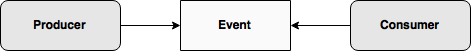
\includegraphics[scale=0.65]{chap3/images/event.png}
%     % event.png: 472x52 pixel, 72dpi, 16.65x1.83 cm, bb=0 0 472 52
%   \end{center}
%   \caption{Event}
%   \label{fig:event}
% \end{figure}
 %An event is a notification that a happening of interest has occurred \cite{glossary}. Examples are a purchase order, an email confirmation of an airline reservation, a stock tick message that reports a stock trade, a message that reports a sensor reading or a smart meter alarm. 
 
 \subsection{Event type}
 An event type is an expression that characterizes a class of significant facts (events) and the context under which they occur. Facts of the same nature are denoted by events that have the same type. 
 %Event types are characterized by an event model.
 An event model gives concepts and general structures used to represent event types.  
 
According to the complexity of the event model, the event types are represented as sequences of strings \cite{Yuhara1994}, regular expressions \cite{Bailey1994} or as expressions of an event algebra \cite{Chakravarthy1994, Gatziu1994, Collet96}. Other models represent an event type as a collection of parameters or attributes, allowing the type itself to contains implicitly the content of the message. This model is useful when we need to reason about events content. For example, $MeterAlarm\ :\ \langle idMeter:string, voltage:real, current:real \rangle$ is an event type that represents a smart meter reading, where the current and voltage values observed are represented by attributes named \textit{voltage} and \textit{current}.\\
Event composition, or specifically event streams composition supports the idea of performing operations on events. Some of those operations needs to access the events content (see Section \ref{ch3:sec2}). 
%The set of operations applicable to events depends on the capacity of the underlying event model to expose the content of events. Event models that expose events content yield to more expressive event composition. 
For that reason, we represent an event type as a tuple type:\\
$EventType : \langle A_1 : D_1, ..., A_n : D_n\rangle.$ \\
The definition of an event type includes the attributes presented in Table \ref{tab:evtAttributes}. The \textit{producerID} attribute refers to the id of the entity that produced the event occurrence. The \textit{detectionTime} attribute refers to the time at which the event occurrence has been detected by a source. The \textit{productionTime} attribute refers to the time at which the event has been produced (as a result of processings on others events) by an event-processing unit. The \textit{notificationTime} attribute refers to the time at which the event is notified to interested consumers. The \textit{receptionTime} attribute refers to the time at which an interested consumer receives the event. In addition to those attributes that are common to all event types, each event type includes other attributes that capture the data that are particular to this event type. For example, a \textit{MeterAlarm} event type is defined as $MeterAlarm\ :\ \langle$\textit{producerID : string,\ detectionTime : time,\ productionTime : time,\ notificationTime : time, receptionTime : time, voltage : real, current : real}$\rangle$.
\\In addition to attributes presented in Table \ref{tab:evtAttributes}, the \textit{MeterAlarm} event type includes the attributes  \textit{idMeter:string, voltage:real, current:real} that represents data that are specific to the MeterAlarm event type. In the rest of this document, we will refer to the attributes presented in Table \ref{tab:evtAttributes} as \textit{header attributes}. For writing simplicity, we will sometimes omit the header attributes in the description of event types and occurrences, when they are not relevant for the topic under consideration. For example, the $MeterAlarm$ event type previously defined can be simply defined as $MeterAlarm\ :\ \langle voltage: real,\ current: real\rangle$.  

\definecolor{tcB}{rgb}{1,1,1}
\definecolor{tcA}{rgb}{0,0,0}
\begin{table}[h!]
\begin{center}
\begin{tabular}{ll}
% use packages: color,colortbl
\rowcolor{tcA}
\textbf{\textcolor{tcB}{Name}} & \textbf{\textcolor{tcB}{Domain}}\\
%\rowcolor{tcA}
%typeName & String\\
%\rowcolor{tcA}
producerID & string\\
%\rowcolor{tcA}
detectionTime & time\\
productionTime & time\\
%\rowcolor{tcA}
notificationTime & time\\
receptionTime & time\\
%\rowcolor{tcA}
%context & Set<Attribute>
\end{tabular}
\caption {Event types attributes}
\label{tab:evtAttributes}
\end{center}
\end{table}
\subsubsection{Event occurrence}
 An event occurrence (or simply event) $e$ is an instance of an event type \textit{EventType}, that is $e\ \equiv \ EventType$. For example, considering the  previously defined event type \textit{MeterAlarm}, $e=\langle 'meter5',\ 1,\ 1,\ 2,\ 4,\ 9,\ 1 \rangle$ is an event instance produced by producer \textit{meter5}, at time 1, notified at time 2, received at time 4, for which the voltage and current values are 9 and 1 respectively. 
 
% \subsection{Simple event type, complex event type}
% Event types can be classified as simple event types that describe elementary facts, and complex event types that describe complex situations by event combinations (see Figure \ref{fig:eventtype}). 
% \begin{figure}[H]
%   \begin{center}
%     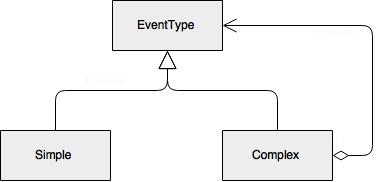
\includegraphics[scale=0.5]{chap3/images/eventType.jpg}
%     % event.png: 472x52 pixel, 72dpi, 16.65x1.83 cm, bb=0 0 472 52
%   \end{center}
%   \caption{Classification of event types}
%   \label{fig:eventtype}
% \end{figure}
% 
% %\subsubsection{Simple event type}
% Event producers produces of a simple event type. Simple event instances are not generated as a result of processing others events.
% 
% %\subsubsection{Complex event type}
% %\label{ch3:sec2.3.2}
% Complex event types represent situations (relevant or critical) that can be inferred from the occurrences of others events. Complex events are produced by processing other events. Event processing operators are defined in Section \ref{ch3:sec2.3.3}.
 \subsection{Event streams}
  An event stream is a continuous, append-only sequence of events $\{e_1,\ ...,\ e_n\}$.
  We note $Stream(s, T)$ the stream of events of type T generated by the source s. That is,
  $Stream(s, T) = \{e_1,\ ...,\ e_n\ |\ \forall e_i,\ e_i \equiv T\ \bigwedge\ e_i.producerID = s\}$.
  If $S$ is a set of sources, then $\{\ \bigcup  stream(s,T),\ s\ \in\ S\}$ defines a stream of events of type T, denoted $Stream(T)$.
 \section{Stream based composition operators}
 \label{ch3:sec3}
 %\subsection{Event streams}
%  An event stream is a continuous, append-only sequence of events. We note $Stream(s, T)$ the stream of events of type T generated by the source s. If S is a set of sources, then $\{\bigcup  stream(s,T), s \in S\}$ defines a stream of events of type T, denoted $Stream(T)$. 
 %Complex events are produced by composing event streams. 
 Event stream composition operators specify the types of operations that can be performed on event streams. An event stream composition operator $op$ takes one or many input event streams of a given type, and produces an output stream of a given type (see Figure \ref{fig:op}). In the following, we  adopt the notation $ES_i$ to denote the event stream of type $E_i$, that is $ES_i\ =\ Stream(E_i)$. 
 \begin{figure}[H]
  \begin{center}
    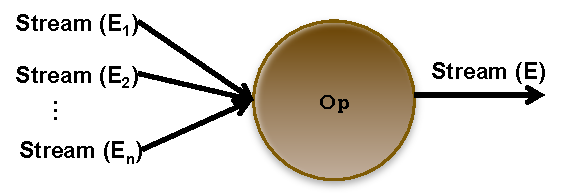
\includegraphics[scale=0.65]{chap3/images/op.pdf}
    % event.png: 472x52 pixel, 72dpi, 16.65x1.83 cm, bb=0 0 472 52
  \end{center}
  \caption{Operator synopsis}
  \label{fig:op}
\end{figure}
Event stream composition operators considered here are : filter, logic operators, sequence, window operators, aggregation operators, selection operator and flatten.  
  \subsection{Filter}
  The \textit{filter} operator selects events in an input stream that satisfy a given predicate. The \textit{filter} operator is denoted $filter_P (ES_i)$. It receives as parameters one input stream $ES_i$ and a predicate $P$.
  The predicate P is defined according to the following rules:
  \begin{itemize}
   \item $A_i\ \theta\ v_i$ is a predicate, where
      \subitem- $A_i$ is the name of an attribute of $E_i$, that is $\exists \hat{t_j}$ such that $\hat{t_j}$ is an attribute type of $E_i$ and $name(\hat{t_j})\ =\ A_i$ 
      \subitem- $\theta\ \in\ \{<,\ >,\ =,\ \leq,\ \geq\}$ is a comparison operator,
      \subitem- $v_i\ \in \llbracket \hat{t_j}\rrbracket$ is a value. 
    \item if $P_1$ and $P_2$ are predicates, then
      \subitem- $P_1\ \bigwedge\ P_2$ is a predicate. The symbol $\bigwedge$ denotes the conjunction.
      \subitem- $P_1\ \bigvee\ P_2$ is a predicate. The symbol $\bigvee$ denotes the disjunction.
  \end{itemize}
 The output of the filter operator is an event stream having the same type as $E_i$. Its output is defined as
 $filter_P(ES_i) = \{e_j\ \mid\ e_j\ \in\ ES_i\ \bigwedge\ P(e_j)\ =\ true\}$.
 % The filter operator produces an event $e$ in the output event stream each time an event $e$ in the input stream satisfies the predicate $P$, that is if $P(e)= true$.
  \\ For example, let's consider the event type $E_i\ =\ MeterMeasure:\langle$ \textit{meterID : string, realPower : double}$\rangle$\footnote{We omitted the header attributes} and some event instances of type $E_i$, $e_1=\langle``meter1``, 7\rangle$, $e_2=\langle``meter1``, 5\rangle, e_3=\langle``meter1``, 4\rangle, e_4=\langle``meter1``, 6\rangle$. 
  \\Let's also consider the event stream $ES_i$ \textit{=Stream(MeterMeasure)} = $\{e_1, e_2, e_3, e_4, ... \}$. 
  \\Then, $filter_{realPower > 5}(ES_i)= \{e_1, e_4, ... \}$. Events $e_2$ and $e_3$ have been filtered out by the filter operator since they don't satisfy the predicate ``realPower > 5``.
 %\subsection{Logic operators}
 %Logic operators produce an event stream based on the occurrence of events in input streams. They are used to test specific pattern of occurrences of event types.
 
 \subsection{Disjunction}
 The disjunction operator merges the input streams into one output stream. The disjunction operator is denoted $OR(ES_1, ES_2, …, ES_n)$. 
 The output of the disjunction operator is an event stream of type $E_1\oplus E_2 ...\oplus E_n$, defined as
 $OR(ES_1, ES_2 ..., ES_n) = \{e_j\ \mid\ \exists i\ \in\ [1..n],\ e_j\ \in\ ES_i\}$ = $\bigcup ES_i,\ i\ \in\ [1..n]$.
 The disjunction operator produces events in the output stream at the occurrence of events in any of the input streams $ES_i,\ i\ \in\ [1..n]$. 
 %An event $e$ is produced in the output stream if an instance $e_i$, of any input stream $ES_i$ occurs. The context of the complex event $e$ contains all occurrences $e_i$ that occur. 
For example, let's consider the event streams $ES_1$ and $ES_2$ in Figure \ref{fig:op_or_exple}.
%types \textit{MeterMeasure} and \textit{MeterAlarm} denoting respectively a measure and an alarm generated by a smart meter. 
%\\Let's consider $ES_1 = Stream(MeterMeasure)$ and $ES_2 = Stream(MeterAlarm)$. Then, $OR(ES_1, ES_2)$  denotes the event stream containing measure and alarm events.
In this example, the output of $OR(ES_1, ES_2)$ is the sequence $\{e_{1,1}, e_{2,1}, e_{2,2}, e_{1,2}, ...\}$.
\begin{figure}[h]
  \begin{center}
    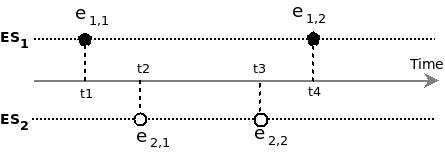
\includegraphics[scale=0.65]{chap3/images/orExample.jpeg}
    % event.png: 472x52 pixel, 72dpi, 16.65x1.83 cm, bb=0 0 472 52
  \end{center}
  \caption{Example situation 1. The time associated to events represents the time at which the events are received by the operator.}
  \label{fig:op_or_exple}
\end{figure}
\subsection{Conjunction}
  The conjunction operator is used to ensure that at least one event occured in all input streams. The conjunction operator is  denoted $AND(ES_1, ES_2, …, ES_n)$. 
   The output of the disjunction operator is an event stream of type $A\ :\ \langle context\ :\ \{E_1\oplus E_2\oplus ... \oplus E_n\} \rangle$\footnote{We omitted the header attributes}, defined as follows:
    $e\ \in\ AND(ES_1, ..., ES_2)$ iff $\forall i\ \in\ [1..n],\ \exists e_{i,j}\ \mid\ e_{i,j}\ \in\ ES_i$. The \textit{context} attribute is defined as follows: \textit{e.context} = $\{e_{i,j}\ \mid\ \forall i, e_{i,j}\ \in\ ES_i\}$.    
  %It produces events in the output stream at the occurrence of events in all of the input streams $ES_i, i \in \{1, 2, …,n\}$. 
  \\In other words, an event $e$ is produced in the output stream if events $e_1, e_2, …, e_n$ occur respectively in input streams $ES_1, ES_2, …, ES_n$, regardless their occurrence order. The attribute \textit{context} of the event $e$ contains all events $e_1, e_2, …, e_n$.
 For example, by considering again the event streams $ES_1$ and $ES_2$ in Figure \ref{fig:op_or_exple}, the output of $AND(ES_1, ES_2)$ will be:
 \begin{itemize}
  \item An event $e_1$ at time t2 with the event parameters $e_{1,1}$ and $e_{2,1}$, such that $e_1.context=\{ e_{1,1}$, $e_{2,1}\}$
  \item An event $e_2$ at time t4 with the event parameters $e_{2,2}$ and $e_{1,2}$, such that $e_2.context=\{ e_{2,2}$, $e_{1,2}\}$.
 \end{itemize}
%  \begin{figure}[h]
%   \begin{center}
%     \includegraphics[scale=0.65]{chap3/images/andExample.jpeg}
%     % event.png: 472x52 pixel, 72dpi, 16.65x1.83 cm, bb=0 0 472 52
%   \end{center}
%   \caption{Example situation 2}
%   \label{fig:op_and_exple}
% \end{figure}
 \subsection{Sequence}
 The sequence operator captures precedence order of events in input streams. The sequence operator is denoted $SEQ(ES_1, ES_2, …, ES_n)$, and receives two or more input event streams $ES_1, ES_2, … ES_n$. 
  The output of the disjunction operator is an event stream of type $A\ :\ \langle context\ :\ \{E_1\oplus E_2\oplus ... \oplus E_n\} \rangle$\footnote{We omitted the header attributes}, defined as follows:\\
$e\ \in\ SEQ(ES_1, ..., ES_2)$ iff $\ \exists\ e_{1}\ \in\ ES_1, ..., e_{n}\ \in\ ES_n\ \mid\ \forall i\ \in\ [1..n-1],\ e_{i}.receptionTime < e_{i+1}.receptionTime$.
\\The \textit{context} attribute contains the set of events $e_i$ that occur. That is, \textit{e.context} = $\{e_{i}\ \mid\ e_{i}$ occurred in $ES_i, \forall i\ \in\ [1..n]\}$.
  
  In other words, the sequence operator produces an event $e$ in output stream each time instances $e_1$ in $ES_1$, $e_2$ in $ES_2$,…, $e_n$ in $ES_n$ are received in the specified order. 
 Then, sequence denotes that $\forall i$, occurrence $e_i$ “is received before” occurrence $e_{i+1}$. 
 %This implies that the reception time of event $e_1.receptionTime < e_2.receptionTime < …< e_n.receptionTime$.
 The context attribute of the event $e$ contains all events $e_1$ and $e_2$, …, $e_n$. 
 For example, let's consider the event streams $ES_1$ and $ES_2$ in Figure \ref{fig:op_seq_exple}, the output of $SEQ(ES_1, ES_2)$ will be:
 \begin{itemize}
  \item An event $e_1$ at time t2 with the event parameters $e_{1,1}$ and $e_{2,1}$, such that $e_1.context=\{ e_{1,1}$, $e_{2,1}\}$;
  \item an event $e_2$ at time t5 with the event parameters $e_{1,2}$ and $e_{2,3}$, such that $e_2.context=\{ e_{1,2}$, $e_{2,3}\}$
 \end{itemize}
 \begin{figure}[h]
  \begin{center}
    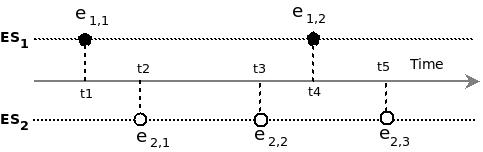
\includegraphics[scale=0.65]{chap3/images/seqExample.jpeg}
    % event.png: 472x52 pixel, 72dpi, 16.65x1.83 cm, bb=0 0 472 52
  \end{center}
  \caption{Example situation 2. The time associated to events represents the time at which the events are received by the operator.}
  \label{fig:op_seq_exple}
\end{figure}
 \subsection{Window operators}
 Window operators partition an event stream into finite parts of the original event stream. Let's consider an input stream $Stream(E)$. We denote by $Stream_f(E)$, a finite part of $Stream(E)$. A window operator applied on $Stream(E)$ results in a stream of finite streams, which we denote $Stream(Stream_f(E))= \{ES_{f,1}, ES_{f,2}, ES_{f,3}, ...\}$.
 The way each finite stream is constructed depends on the window specification, which can be \textit{time-based} or \textit{tuple-based}.
 \subsubsection{Time based windows}
Time based windows define windows using time intervals.
\begin{figure}[h]
  \begin{center}
    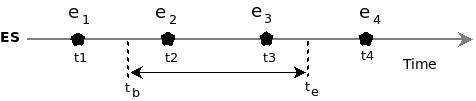
\includegraphics[scale=0.65]{chap3/images/winwithinExample.jpeg}
    % event.png: 472x52 pixel, 72dpi, 16.65x1.83 cm, bb=0 0 472 52
  \end{center}
  \caption{Example situation 3. The time associated to events represents the time at which the events are received by the operator.}
  \label{fig:op_winwithin_exple}
\end{figure}
\begin{itemize} 
\item \textbf{Fixed windows}: $win:within_{(t_b, t_e)}(ES)$. Defines a fixed time interval $[t_b, t_e]$. The output stream contains a single finite event stream $ES_{f,1}$ such that $\forall e \in ES, e \in ES_{f,1}$ iff $t_b \leq e_i.receptionTime \leq t_e $. In the example depicted in Figure \ref{fig:op_winwithin_exple}, the output of $win:within_{(t_b, t_e)}(ES)$ is the finite event stream $\{e_2, e_3\}$ 
\item \textbf{Landmark windows}: $win:since_{t_b}(ES)$. Defines a fixed lower bound time $t_b$. The output stream is a sequence of finite event streams $ES_{f,i}, i \in \{1, 2, …, n\}$, such that each $ES_{f,i}$ contains events $e_i$ received since the time lower bound $t_b$. That is, $\forall i, e \in ES_{f,i}$ iff $t_b \leq e_i.receptionTime$.
In the example depicted in Figure \ref{fig:op_winwithin_exple}, the output of $win:since_{t_b}(ES)$ is the finite event stream $\{e_2, e_3, e_4\}$ 
\item \textbf{Sliding windows}: $win:sliding_{(t_w, t_s)}(ES)$. Defines a time duration $t_w$ and a time span $t_s$. The output stream is a sequence of finite event streams  $ES_{f,i}, i \in \{1, 2, …, n\}$, such that each $ES_{f,i}$ contains events from stream $ES$ produced 
during last $t_w$ time units. The finite event streams in the sequence are produced each $t_s$ time unit. That is, if $ES_{f,i}$ is produced at time t, then $ES_{f,i+1}$ will be produced at time $t+t_s$.
In the example depicted in Figure \ref{fig:op_winsliding_exple}, the output of $win:sliding_{(t_w, t_s)}(ES)$ are the finite event streams $\{e_1, e_2\}$ and $\{e_4\}$.
\begin{figure}[h]
  \begin{center}
    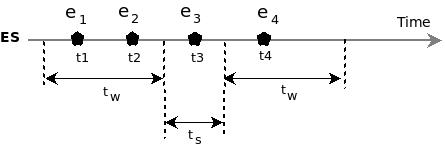
\includegraphics[scale=0.65]{chap3/images/winslidingExample.jpeg}
    % event.png: 472x52 pixel, 72dpi, 16.65x1.83 cm, bb=0 0 472 52
  \end{center}
  \caption{Example situation 4. The time associated to events represents the time at which the events are received by the operator.}
  \label{fig:op_winsliding_exple}
\end{figure}
\end{itemize}
\subsubsection{Size bounded windows}
A size bounded window defines the number of events for each window. We distinguish between size fixed windows and sliding size fixed windows.
\begin{itemize}
 \item \textbf{Fixed size windows}: $win:batch_{nb}(ES)$. Specifies a fixed size \textit{nb} of each finite stream. The output stream is a sequence of finite event streams $ES_{f,i}, i \in \{1, 2, …, n\}$, such that each finite event stream $ES_{f,i}$ contains $nb$ most recent events from $ES$, and are non-overlapping. If we consider the event stream $ES = \{e_1, e_2, e_3, e_4, e_5, e_6, …\}$, $win:batch_3(ES)$ will result in finite event streams $\{ES_{f,1}, ES_{f,2},...\}$ such that $ES_{f,1} = \{ e_1, e_2, e_3\}$, $ES_{f,2} = \{ e_4, e_5, e_6\}$, and so on. 

 \item \textbf{Moving fixed size windows}: $win:mbatch_{(nb, m)}(ES)$. Defines a fixed size $nb$ of each finite stream, and a number of events $m$ after which the window moves. The output stream is a sequence of finite event streams $ES_{f,i}, i \in \{1, 2, …, n\}$, such that each $ES_{f,i}$ contains $nb$ most recent events from $ES$. $ES_{f,i+1}$ is started after $m$ events are received in $ES_{f,i}$ (moving windows). As result, an event instance may be part of many finite event streams. This is the case if $m \leq nb$. For example, if we consider windows of size nb=3 moving after each m = 2 events, that is $win:mbatch_{(3, 2)}(ES)$, the event stream $ES = \{ e_1, e_2, e_3, e_4, e_5, e_6, e_7, …\}$ will be partitioned into finite event streams $\{ES_{f,1}, ES_{f,2}, ES_{f,3} , …\}$ such that $ES_{f,1}=\{e_1, e_2, e_3\}$, $ES_{f,2} = \{ e_3, e_4, e_5\}$, $ES_{f,3} = \{e_5, e_6, e_7\}$, and so on.
\end{itemize}

\subsection{Aggregation operators}
Applied on a stream of finite streams $Stream(Stream_f(E))= \{ES_{f,1}, ES_{f,2}, ES_{f,3}, ...\}$, an aggregator operator $aggregate_{attr,\ aggrAttr}(Stream(Stream_f(E)))$ computes for each finite stream $ES_{f,i}, i \in \{1, 2, …, n\}$, the aggregated value of the attribute \textit{attr} over events occurrences in $ES_{f,i}$.
\\The attribute \textit{attr} is the name of an attribute of $E$, that is $\exists \hat{t_j}$ such that $\hat{t_j}$ is an attribute type of $E$ and $name(\hat{t_j})\ =\ attr$.  
\\The output is a event stream of type $A\ :\ \langle aggrAttr\ :\ D \rangle$\footnote{We omitted the header attributes} 
where $D=def(\hat{t_j})$. 
\\ Aggregate operators include \textit{max, min, count, avg} and \textit{sum}. 
\begin{itemize}
 \item The $max$ operator compute the maximum value of the attribute over the event instances in $ES_{f,i}$.
 \item The $min$ operator compute the minimum value of the attribute over the event instances in $ES_{f,i}$.
 \item The $count$ operator compute the number of event instances in $ES_{f,i}$ with the specified attribute.
 \item The $avg$ operator compute the average value of the attribute over the event instances in $ES_{f,i}$.
 \item The $sum$ operator compute the sum of the attribute's values over the event instances in $ES_{f,i}$.
\end{itemize}

\subsection{Selection operators}
A selection operator takes as input a stream of finite streams $Stream(Stream_f(E))= \{ES_{f,1}, ES_{f,2},...\}$ and produce as output an event stream of type $E$, with values ${e_1, e_2, … }$ such that for all i, each $e_i$ is a selection of a particular event from $ES_{f,i}$. The choice of that particular occurrence depends on the selection operator: %[GD93, GD94]:
\begin{itemize}
 \item \textbf{ First occurrence}: $first (Stream(Stream_f(E)))$. \\
For each finite stream $ES_{f,i}, i \in \{1, 2, …, n\}$, selects the first event occurrence. For example, if we apply the first operator to the stream of finite streams $\{\{e_1, e_2\}$, $\{ e_3, e_4, e_5, e_6\}$, $\{ e_7, e_8\},…\}$, we obtain as output the stream $\{e_1, e_3, e_7, …\}$.
   \item \textbf{Last occurrence}: $last (Stream(Stream_f(E)))$. \\
For each finite stream $ES_{f,i}, i \in \{1, 2, …, n\}$, selects the last event occurrence. For example, if we apply the last operator to the stream of finite streams $\{\{e_1, e_2\}$, $\{ e_3, e_4, e_5, e_6\}$, $\{ e_7, e_8\},…\}$, we obtain as output the stream $\{e_2, e_6, e_8, …\}$.
\end{itemize}
\subsection{Flatten}
The flatten operator is denoted $flatten(Stream(Stream_f(E)))$.
The \textit{flatten} operator takes as input a stream of finite event streams $Stream(Stream_f(E))= \{ES_{f,1}, ES_{f,2}, ES_{f,3}, ...\}$  and produces as output an event stream of type $E$, which contains the concatenation of events in $ES_{f,1}, ES_{f,2}, ES_{f,3}$, and so on. 
For example, if we consider the stream of finite streams $\{\{e_1\}, \{e_2, e_3\}, \{e_4, e_5, e_6\}, …\}$, the flatten operator produces the output stream $\{e_1, e, e_2, e_3,e, e_4, e_5, e_6, e, …\}$ where $e$ is a special “empty” event that indicates the end of each finite stream in the output stream. We assume that for all event type $E$, the empty event $e$ satisfies $e\ \equiv \ E$.

%\section{Selection policy}
%\label{ch3:sec4}
% In general, stream based operators process selects one or more input event streams and produce as output one event stream.
% In some cases, an operator can receive many instances of input events can be of events 
% The production of one event in the output stream 
% In general, stream-based operators select some events in input str
% perfom event per event, as event are arriving on input event streams. This is the case for the filter operator, the For example, In some cases,
% xxxxxxxxxxxxxxxxxxxxxxxxxxxxxxxxxxxxxxxxxxxxxxxxxxxxxxxxxxxxxxxxxxxxxxxxxxxxxxxxxxxxxxxxxxxxxxxxxxxxxxxxxxxxxxxxxxxxxxxxxxxxxxxxxxxxxxxxxxxxxxxxxxxxxxxxxxxxxxxxxxxxxxxxxxxxx
%There are ambiguous situations where an operator has to select between many event in input streams in order to produce a complex event. For example, consider the situation depicted in Figure \ref{fig:selectionpolicy} where the \textit{and} operator is performed on two event streams A and B. Suppose that two event occurrences $a_1$ and $a_2$ are received from input stream A at time $t_1$ and $t_2 > t_1$ respectively. According to the operator definition, a complex event has to be produced in the output stream when occurrences from input streams A and B are received. So, at time $t_2$, there is nothing produced in the output. Now let's suppose that an occurrence $b_1$ is received from input stream B at time $t_3 > t_2$. Now, the \textit{and} operator should produce a composite event in the output. For that, it must be specified which occurrence between $a_1$ and $a_2$ should be considered for the construction of the complex event. It is the goal of selection policies, to specify the events to be selected in such situations. The event selection policies are classified in recent, chronologic,  continuous and cumulative.

%\begin{figure}[H]
 % \begin{center}
  %  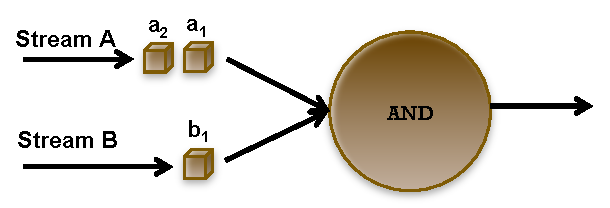
\includegraphics[scale=0.65]{chap3/images/selectionpolicy.pdf}
    %% event.png: 472x52 pixel, 72dpi, 16.65x1.83 cm, bb=0 0 472 52
  %\end{center}
  %\caption{Example situation where a selection policy should be applied}
  %\label{fig:selectionpolicy}
%\end{figure}
%\begin{description}
 % \item[Recent]  Only the newest event occurrence is selected. In the example depicted in Figure \ref{fig:selectionpolicy}, the event $a_2$ is selected between $a_1$ and $a_2$.
 % \item[Chronologic]  Only the oldest event occurrence is selected. In the example depicted in Figure \ref{fig:selectionpolicy}, the event $a_1$ is selected between $a_1$ and $a_2$.
 % \item[Continuous] All the event occurrences are selected. In the example depicted in Figure \ref{fig:selectionpolicy}, the event $a_1$ and $a_2$ are selected. As result, two complex events are produced in the output stream, with event parameters \{$a_1$, $b_1$\} and \{$a_1$, $b_2$\} respectively.
 % \item[Cumulative]  All the event occurrences are accumulate in order to produce the complex event. In the example depicted in Figure \ref{fig:selectionpolicy}, the event $b_1$ is combined with both events $a_1$ and $a_2$.
% \end{description}

 \section{Event streams composition}
 \label{ch3:sec5}
 %\subsection{Event stream composition expression}
 Stream based operators can be chained in order to produce complex event streams that capture particular situations.
 This is called event stream composition.
 An event stream composition is expressed by an event stream composition expression.
An event stream composition expression is defined as:
\begin{itemize}
 \item $A\ =\ Op(ES_1,...ES_n)$ is an event stream composition expression named $A$, where $Op$ denotes a stream based operator and $\forall i\ \in\ [1..n]$, $ES_i$ denotes an event stream.
 \item $A\ =\ Op_1(Op_2(...(Op_n(A_1,...A_m))...))$ where $\forall i\ \in\ [1..n],\ \forall j\ \in\ [1..m]$, $Op_i$ is a stream based operator and $A_j$ is an event stream composition expression.
 \end{itemize}
 The event stream composition expression defines an event stream named $A$
 An event stream composition expression A defines an event stream with the same name $A$. 
For example, if we consider the event type $MeterMeasure:\langle$ \textit{meterID : string, realPower : double}$\rangle$ and the event stream $ES=Stream(MeterMeasure)$, we can define an event stream \textit{ComplexStream} that computes the aggregated real power of meter \textit{'AMI100'} between time 10 and 50 as follows:
 \\$ComplexStream=avg_{realPower,\ avgP}$\textit{(win:within(}$filter_{meterID='AMI100'}(ES)$\textit{, 10, 50))}.
 The definition of the \textit{ComplexStream} starts by filtering the event stream $ES$ on the predicate \textit{meterID='AMI100'}. Then, the result is used to compute a fixed windows (\textit{win:within}) of events between time 10 and 50. The output stream, which is a finite stream is then aggregated on the attribute \textit{realPower}. The aggregated value can be retrieved by accessing the \textit{avgP} attribute of the event $e$ in the \textit{ComplexStream} output stream.
 %Complex events are defined by consumers in order to state the situations they are interested in. Those situations can be described in terms of operations that have to be applied to event streams in order to obtain the desired result.   
% A complex event is represented as an \textit{event composition graph} (see Figure \ref{fig:ecg}). An event composition graph is a structure that identifies the event streams to be processed with the operation chain to be performed on them. In a more formal way, an event composition graph is a direct acyclic graph (DAG) $G=<\mathcal{N}, \mathcal{S}>$, where $\mathcal{N}= \{P \cup O\}$ consists in a set of terminal nodes $P$ and a set of non-terminal nodes $O$, and a set of edges $\mathcal{S}$. Terminal nodes $P$ represent input stream producers and non-terminal nodes $O$ represent stream based operators. The edges $\mathcal{S}$ represent event streams. From an end user point of view, an event composition graph can be specified using either a graphical user interface, or programmaticaly. 
 %We  In this thesis, we only consider their internal representation as DAGs.% with less focus on how such DAG can be defined from an end user point of view.   
% \begin{figure}[H]
 % \begin{center}
  %  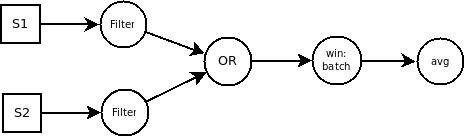
\includegraphics[scale=0.65]{chap3/images/ecg.jpg}
    % event.png: 472x52 pixel, 72dpi, 16.65x1.83 cm, bb=0 0 472 52
  %\end{center}
  %\caption{Event composition graph}
  %\label{fig:ecg}
%\end{figure}
  %\subsection{Valid event stream composition expression}
  
  An event stream composition expression must be well formed. More precisely, the input of each stream based operator $Op_i$ implicated in the event stream composition expression must be consistent with the operator definition. For example, the input of an aggregate operators is a stream of finite streams, which can be computed using windows operators as in the \textit{ComplexStream} example. Moreover, the result of a windows operator, which is a stream of finite event streams, cannot be given directly as input to a filter operator as in the expression $FilteredStream=filter_P(win:sliding_{(t_w,t_s)}(ES))$. 
  This is due to the fact that the filter operator takes as input an event stream, an not a stream of finite event streams. In order to be consistent with the filter operator definition, the \textit{FilteredStream} expression can be written $FilteredStream=filter_P(flatten(win:sliding_{(t_w,t_s)}(ES)))$.    
 \section{Conclusion}
In this chapter, we presented a model for event streams composition.
We focused on the definition of concepts that are manipulated by an event stream composition system.
First, we presented the concepts of event, event types, event occurrence and event streams.
Then, we presented operators applicable to event streams with their associated semantic. 
After that, we introduced event stream composition and event stream composition expressions, as mechanisms for combining stream based operators in order to produce complex event streams.
%And finally, we presented some QoS dimensions applicable to an event composition, and how they can be specified using QoS expressions. 

In the next chapter, we will go one step forward, by presenting how the presented model can be leveraged to define an approach for distributed event streams composition that deals with QoS.